\documentclass[conference]{IEEEtran}
\IEEEoverridecommandlockouts

\usepackage[utf8]{inputenc}
\usepackage[T1]{fontenc}
\usepackage{amsmath,amssymb}
\usepackage{graphicx}
\usepackage{booktabs}
\usepackage{array}
\usepackage{multirow}
\usepackage{url}
\usepackage{tikz}
\usetikzlibrary{positioning,arrows.meta,fit,backgrounds,calc}
\usepackage[hidelinks]{hyperref}

% Turkish caption labels (Figure / Table)
\renewcommand{\figurename}{Şekil}
\renewcommand{\tablename}{Tablo}

\begin{document}

\title{Doğrudan Sürüş Kontrolünün Sınırlarını Ölçmek:\\ CARLA Ortamında BEV, Ego-State ve Çok-Kamera Füzyonuna Dayalı Hibrit Bir Mimari}

\author{
\IEEEauthorblockN{Halil İbrahim Şenaydın}
\IEEEauthorblockA{Bilgisayar Mühendisliği Anabilim Dalı, Yüksek Lisans Programı\\
\textit{(Atatürk Üniversitesi)} \\
halilsenaydin@gmail.com}
}

\maketitle

% SECTION - ABSTRACT
\begin{abstract}
End-to-end otonom sürüşte sensör verisinden doğrudan kontrol komutu üretmek, hem mimari hem istatistiksel açıdan zorlu bir regresyon problemidir; özellikle brake, throttle ve steer sinyallerinin aynı anda kestirilmesi gerektiğinde. Modern çok-modlu füzyon çalışmaları kontrolü çoğunlukla doğrudan değil, waypoint kestirimi üzerinden ürettiği için, tam bir çok-modlu füzyon mimarisinin üç kontrol sinyalini doğrudan tahmin ettiğinde ne ölçüde başarılı olduğu yeterince incelenmemiştir. Bu çalışmada, bu soru ele alınmış ve CARLA simülatöründe toplanmış çok-modlu bir otopilot veri kümesi üzerinde brake, throttle ve steer değerlerini tek geçişte kestiren hibrit bir model önerilmiştir. Model üç branch içerir: LiDAR nokta bulutundan üretilen BEV temsilini EfficientNet-B0 backbone'u ve ConvLSTM ile spatio-temporal olarak kodlayan vision branch, sayısal ego-state dizisini bir GRU ile işleyen state branch ve karar anındaki dört kamera görüntüsünü (ön, sol-ön, sağ-ön ve arka) paylaşımlı bir EfficientNet-B1 ile kodlayan image branch. Üç branch late fusion ile birleştirilir ve çıkış başlıkları kontrol sinyallerini doğal aralıklarında üretir. Aynı veri kümesi üzerinde yalnızca skaler özniteliklerle eğitilen bir MLP temel modeliyle karşılaştırma yapılmış, ayrıca her bileşenin katkısı tek değişkenli bir ablasyon çalışmasıyla ayrıştırılmıştır. Hibrit model test kümesinde 0,9221 genel $R^2$ değeriyle temel modelin 0,8605 değerini geçmiş; en büyük kazanım, uzamsal ve görsel bilginin en belirleyici olduğu steer kanalında gözlenmiştir. Brake kanalı 0,9759 $R^2$ ile en güvenilir tahmin edilen sinyal olmuş ve bu sonucun dengesizlikten kaynaklanmadığı, dengeli aktiflik oranı ve aktif-örnek analiziyle gösterilmiştir. Değerlendirme open-loop koşullarında yapılmış olup, doğrudan kontrol paradigmasının bilinen closed-loop kırılganlıkları ayrıntılı biçimde tartışılmıştır.
\end{abstract}

\begin{IEEEkeywords}
autonomous driving, imitation learning, sensor fusion, bird's-eye view, multi-camera fusion, ConvLSTM, CARLA, control prediction, multimodal learning
\end{IEEEkeywords}

% SECTION - INTRODUCTION
\section{Giriş}

Otonom araçların karar yığını geleneksel olarak algılama, konumlama, planlama ve kontrol biçiminde ayrık modüllere bölünür. Bu ayrıştırma her bileşenin bağımsız geliştirilmesine olanak tanısa da, modüller arasında biriken hata ve her aşamanın elle ayarlanması ihtiyacı sistemin bütününü kırılgan kılar. End-to-end öğrenme bu kırılganlığı azaltmayı amaçlar ve ham sensör verisinden sürüş davranışına uzanan eşlemeyi tek bir türevlenebilir ağa yükler. CARLA \cite{Dosovitskiy17} gibi yüksek doğruluklu simülatörlerin yaygınlaşması bu yaklaşımın güvenli ve tekrarlanabilir biçimde denenmesini mümkün kılmış, son yıllarda da olgun bir literatür ortaya çıkmıştır \cite{Chen24Survey}.

Bu çalışmanın odağı, çok-modlu sensör verisinden aracın üç temel kontrol sinyalini, yani brake, throttle ve steer değerlerini doğrudan kestiren bir model kurmaktır. Problemin önemi iki yönden anlaşılabilir. Bu üç sinyal aracın boylamsal ve yanal hareketini birlikte belirler; dolayısıyla gerçekçi bir sürüş davranışı ancak üçünün uyumlu biçimde üretilmesiyle ortaya çıkar. Aynı zamanda bu sinyallerin istatistiksel davranışı birbirinden hayli farklıdır. Steer çift yönlüdür ve yolun geometrisini yakından izler. Brake çoğu karede ya tümüyle devrededir ya da hiç yoktur, dolayısıyla iki kutuplu bir yapı sergiler. Throttle ise sürekli değer alır ve seyir ile hızlanma arasında birden çok çalışma noktasına yayılır. Modelin aynı temsilden hem keskin bir frenleme kararına hem de yumuşak bir gaz kestirimine ulaşması beklendiğinden, üç sinyali tek bir ağda aynı anda öğrenmek başlı başına bir zorluktur.

End-to-end CARLA literatürü, ürettiği çıktının türüne göre iki çizgide ilerler. Birinci çizgi kontrolü doğrudan üretir. CIL \cite{Codevilla18}, görüntüden steer ve hızlanma değerlerini navigasyon komutuna göre dallandırarak öğrenir. Ardılı CILRS \cite{Codevilla19}, ImageNet üzerinde önceden eğitilmiş bir ResNet \cite{He16ResNet} backbone'una açık bir hız tahmin kolu ekleyerek brake, throttle ve steer'i birlikte regresyonla kestirir ve başarımını NoCrash benzeri benchmark'larda sürüş başarı oranıyla bildirir. Learning by Cheating \cite{Chen19LBC} önce BEV gören ayrıcalıklı bir öğretmen eğitir, sonra bu bilgiyi yalnızca kameralı bir öğrenciye aktarır. Roach \cite{Zhang21Roach}, BEV gören bir reinforcement learning uzmanını taklit eden bir öğrenci politikası kurar ve kontrolü olasılıksal bir dağılım olarak modeller. Bu çalışmaların ortak yanı, başarımı $R^2$ gibi open-loop regresyon hatalarıyla değil, Driving Score ve route completion gibi closed-loop sürüş metrikleriyle raporlamalarıdır.

İkinci çizgi kontrolü dolaylı üretir. Model gelecekteki trajectory'yi waypoint'ler hâlinde kestirir, ardından bir PID denetleyici bu noktaları sürüş komutlarına çevirir. TransFuser \cite{Prakash21Transfuser,Chitta23Transfuser} kamera ve LiDAR-BEV özelliklerini transformer attention mekanizmasıyla kaynaştırarak waypoint üretir ve CARLA Leaderboard ile Longest6 üzerinde güçlü Driving Score değerleri elde eder. LAV \cite{Chen22LAV} çevredeki tüm araçların gözlemlerinden öğrenerek veri verimliliğini artırır. InterFuser \cite{Shao22Interfuser} çok kameralı ve LiDAR girdisini yorumlanabilir bir güvenlik haritasıyla birleştirir. ST-P3 \cite{Hu22STP3} yalnızca kameradan spatio-temporal bir BEV temsili kurar, ReasonNet \cite{Shao23ReasonNet} ise zamansal ve küresel akıl yürütmeyle yoğun trafikli sahneleri ele alır. TCP \cite{Wu22TCP} iki çizgiyi tek bir ağda buluşturur: bir trajectory dalı ile bir doğrudan kontrol dalını birlikte eğitir ve tek kamerayla, çok sensörlü yöntemleri geride bırakarak 2022 CARLA sürüş yarışmasının en yüksek skorlarına ulaşır. Bu yöntemler de başarımlarını closed-loop sürüş metrikleriyle bildirir; bu nedenle sonuçları, bu çalışmanın open-loop regresyon ölçütleriyle doğrudan kıyaslanamaz.

Modern füzyon çalışmalarının waypoint çıktısına yönelmesinin somut bir gerekçesi vardır. Behavior cloning ile eğitilen bir model yalnızca uzmanın ziyaret ettiği state dağılımını görür. Test sırasında modelin kendi küçük hataları aracı bu dağılımın dışına taşıdığında, model daha önce hiç karşılaşmadığı durumlarla yüzleşir ve hatalar zincirleme büyür. Distribution shift olarak adlandırılan bu olgu nedeniyle, open-loop ölçülen düşük tahmin hatası gerçek sürüş kalitesini garanti etmez. Codevilla ve ark. \cite{CodevillaOffline18} offline hata ile closed-loop başarım arasındaki ilişkinin zayıf olduğunu deneysel olarak göstermiştir. Waypoint temsili, araya giren denetleyici katmanı sayesinde bu kaymaya doğrudan kontrole kıyasla daha dayanıklıdır ve modern füzyon hattının bu temsili tercih etmesinin temel nedeni budur. Doğrudan kontrolün bu sınırlılığı, bu çalışmada bir kusur olarak değil, bilinçli bir inceleme nesnesi olarak ele alınmıştır: amaç, tam çok-modlu füzyonla doğrudan kontrolün ulaşabileceği open-loop başarımı ölçmek ve ortaya çıkan eksikleri bir sonraki tez çalışmasına yön verecek biçimde tespit etmektir.

BEV temsili ve zamansal modelleme tarafında da önerilen yöntemle doğrudan örtüşen çalışmalar vardır. Lift-Splat-Shoot \cite{Philion20LSS} kameradan BEV'e geçişte ImageNet üzerinde önceden eğitilmiş bir EfficientNet backbone'u kullanır. FIERY \cite{Hu21Fiery} aynı backbone ailesini zamansal BEV kestirimiyle birleştirir. ChauffeurNet \cite{Bansal19Chauffeur} rasterleştirilmiş BEV katmanlarını recurrent bir ağla işler, MILE \cite{Hu22MILE} ise BEV temelli bir world model kurar. Önerilen modelin EfficientNet-B0 ve ConvLSTM tabanlı vision branch'i bu çizginin doğrudan devamı niteliğindedir.

Önerilen model birinci çizgiyi, yani doğrudan üç-kontrol regresyonunu benimser; ancak girdi tarafında ikinci çizginin çok-modlu füzyon fikirlerini bir araya getirir. Üç ayrı branch kullanılır. Vision branch, LiDAR nokta bulutundan üretilen BEV temsilini bir EfficientNet-B0 \cite{Tan19EfficientNet} backbone'u ve ConvLSTM \cite{Shi15ConvLSTM} ile spatio-temporal olarak kodlar. State branch, hız ve ivme başta olmak üzere sayısal ego-state dizisini bir GRU \cite{Cho14GRU} ile özetler. Image branch ise karar anındaki dört kamera görüntüsünü (ön, sol-ön, sağ-ön ve arka) paylaşımlı bir EfficientNet-B1 örneğiyle kodlar. Üç branch late fusion ile birleştirilir ve çıkış başlıkları kontrol sinyallerini doğal aralıklarında üretir.

Bu çalışmanın çıkış noktası pratik bir sorudur: tüm sensörleri kullanan bir füzyon mimarisi kurulup kontrol sinyalleri doğrudan kestirildiğinde ne elde edilir? Modern füzyon literatürü doğrudan üç-kontrol regresyonu yerine waypoint kestirimini tercih ettiğinden, bu birleşim yeterince araştırılmamıştır. Bu boşluğu doldurmak ve bir tez çalışmasına zemin hazırlamak amacıyla aşağıdaki katkılar sunulmaktadır:

\begin{itemize}
\item BEV, ego-state ve çok-kamera modalitelerini late fusion ile birleştiren, brake, throttle ve steer'i tek geçişte regresyonla kestiren modüler bir hibrit mimari önerilmekte ve uygulama ayrıntıları bütünüyle paylaşılmaktadır.
\item Aynı veri kümesi üzerinde yalnızca skaler özniteliklerle eğitilen bir MLP temel modeliyle karşılaştırma yapılarak, her kontrol sinyali için spatio-temporal ve görsel modellemenin katkısı niceliksel olarak ölçülmektedir.
\item Önerilen modelin başlıca bileşenlerinin --- çok-kamera image branch'i, image backbone kapasitesi, zamansal modelleme ve ince-ayar stratejisi --- payı, tek değişkenli bir ablasyon çalışmasıyla ayrıştırılmaktadır.
\item Brake, throttle ve steer arasındaki ilişki ile bu sinyallerin BEV, ego-state ve image modaliteleriyle bağlantısı hem mimari hem deneysel kanıtla açıklanmaktadır.
\item Raporlanan başarımın bir sınıf dengesizliği yapaylığı olmadığı, üç sinyal için ayrı ayrı yürütülen aktif-örnek analiziyle doğrulanmaktadır.
\end{itemize}

Ele alınan başlıca yöntemlerin girdi modalitesi, çıkış türü ve backbone açısından özeti Tablo~\ref{tab:related}'de verilmiştir. Bilinen kaynaklar arasında, kullanılan çok-modlu veri kümesi \cite{immanuel_peter_2025} üzerinde hibrit ego-state, BEV ve image füzyonuyla kontrol kestirimi yapan başka bir hakemli çalışma bulunmadığından, niceliksel karşılaştırma temel model ve ablasyonlar üzerinden kurulmuştur.

% TABLE - related-work
\begin{table}[!t]
\caption{End-to-end CARLA yöntemlerinin girdi, çıktı ve backbone özeti}
\label{tab:related}
\centering
\footnotesize
\renewcommand{\arraystretch}{1.1}
\resizebox{\columnwidth}{!}{%
\begin{tabular}{@{}lccc@{}}
\toprule
\textbf{Yöntem} & \textbf{Girdi} & \textbf{Çıkış} & \textbf{Backbone} \\
\midrule
CIL \cite{Codevilla18}        & kamera            & doğrudan kontrol   & CNN \\
CILRS \cite{Codevilla19}      & kamera + hız      & doğrudan kontrol   & ResNet \\
Roach \cite{Zhang21Roach}     & BEV / kamera      & doğrudan kontrol   & CNN \\
TransFuser \cite{Chitta23Transfuser} & kamera + LiDAR & waypoint & ResNet/RegNet \\
LAV \cite{Chen22LAV}          & kamera + LiDAR    & waypoint           & ResNet \\
InterFuser \cite{Shao22Interfuser} & çok kamera + LiDAR & waypoint + güvenlik & CNN + Tr. \\
TCP \cite{Wu22TCP}            & kamera            & waypoint + kontrol & ResNet-34 \\
ST-P3 \cite{Hu22STP3}         & çok kamera        & waypoint           & CNN + BEV \\
\textbf{Bu çalışma}           & BEV + ego + çok kamera & doğrudan kontrol  & EfficientNet-B0/B1 \\
\bottomrule
\end{tabular}%
}
\end{table}

% SECTION - METHOD
\section{Yöntem}

\subsection{Genel Mimari}

Önerilen modelin genel yapısı Şekil~\ref{fig:arch}'de sunulmuştur. Model, birbirinden bağımsız üç encoder branch ve bunların çıktısını birleştiren tek bir fusion başlığından oluşur. Tasarımın arkasındaki temel düşünce, her modalitenin kendi doğasına uygun bir kodlayıcıyla işlenmesi ve karar ancak en sonda, modalite-özgü özetler bir araya getirildikten sonra verilmesidir. Bu late fusion yaklaşımı, early  fusion'a kıyasla iki avantaj sağlar. Her branch kendi alanına özgü önyargılarla, örneğin BEV'in uzamsal yapısı ya da ego-state'in zamansal eğilimi göz önünde bulundurularak ayrı ayrı eğitilebilir; ayrıca bir modalitenin temsil boyutu değiştiğinde diğer branch'ler etkilenmeden korunur.

Model, $T=8$ uzunluğunda bir zamansal pencere üzerinde çalışır. Pencere boyunca her kare için bir BEV tensörü ve bir ego-state vektörü kullanılır; kamera görüntüleri ise yalnızca karar anı için, yani pencerenin son karesi için alınır. Bu asimetri bilinçlidir: BEV ve ego-state, aracın yakın geçmişteki dinamiğini taşıdıkları için zamansal olarak işlenirken, kameralar tek bir anlık çok-görünümlü bağlam olarak değerlendirilir. Karar karesinde dört kamera görünümü birlikte kullanılır; böylece aracın çevresi yalnızca önden değil, yanlardan ve arkadan da kapsanır. Modelin ürettiği çıktı, pencerenin son karesine ait $[\text{brake}, \text{throttle}, \text{steer}]$ kontrol vektörüdür.

% FIGURE - architecture
\begin{figure}[t]
\centering
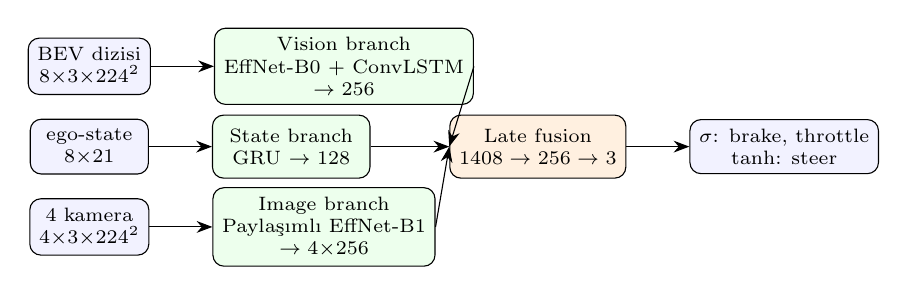
\begin{tikzpicture}[
  font=\scriptsize,
  box/.style={draw,rounded corners,minimum height=6mm,minimum width=15mm,align=center,fill=blue!5},
  enc/.style={draw,rounded corners,minimum height=8mm,minimum width=20mm,align=center,fill=green!7},
  fus/.style={draw,rounded corners,minimum height=8mm,minimum width=22mm,align=center,fill=orange!12},
  >={Stealth[length=2mm]}
]
\node[box] (bev) {BEV dizisi\\$8{\times}3{\times}224^2$};
\node[box,below=3mm of bev] (ego) {ego-state\\$8{\times}21$};
\node[box,below=3mm of ego] (img) {4 kamera\\$4{\times}3{\times}224^2$};

\node[enc,right=8mm of bev] (cnn) {Vision branch\\EffNet-B0 + ConvLSTM\\$\rightarrow 256$};
\node[enc,right=8mm of ego] (gru) {State branch\\GRU $\rightarrow 128$};
\node[enc,right=8mm of img] (icnn) {Image branch\\Paylaşımlı EffNet-B1\\$\rightarrow 4{\times}256$};

\node[fus,right=10mm of gru] (fuse) {Late fusion\\$1408\rightarrow256\rightarrow3$};
\node[box,right=8mm of fuse] (out) {$\sigma$: brake, throttle\\$\tanh$: steer};

\draw[->] (bev)--(cnn);
\draw[->] (ego)--(gru);
\draw[->] (img)--(icnn);
\draw[->] (cnn.east)--(fuse.west);
\draw[->] (gru)--(fuse);
\draw[->] (icnn.east)--(fuse.west);
\draw[->] (fuse)--(out);
\end{tikzpicture}
\caption{Önerilen hibrit mimari. Vision branch BEV'i EfficientNet-B0 ve ConvLSTM ile spatio-temporal olarak kodlar; image branch dört kamera görünümünü paylaşımlı bir EfficientNet-B1 ile kodlar; state branch ego-state'i GRU ile dizisel olarak kodlar. Üç özet late fusion ile birleştirilir.}
\label{fig:arch}
\end{figure}

\subsection{LiDAR'dan BEV Temsiline Dönüşüm}

Ham LiDAR taraması, her biri $(x_n, y_n, z_n, i_n)$ değerlerine sahip $N$ noktadan oluşur. Bu noktalar, aracı merkez alan ve $[-R, R]^2$ düzlemini $S\times S$ ızgaraya bölen bir kuş bakışı tensöre yansıtılır; burada $R=80$~m ve $S=224$ alınmıştır. Bir noktanın piksel indisleri
\begin{align}
c &= \left\lfloor \frac{x - x_{\min}}{x_{\max}-x_{\min}}\,(S-1) \right\rceil, \\
r &= \left\lfloor \frac{y_{\max}-y}{y_{\max}-y_{\min}}\,(S-1) \right\rceil,
\end{align}
ile hesaplanır; $x_{\min}=y_{\min}=-R$ ve $x_{\max}=y_{\max}=R$ değerleri menzili kapsar. Elde edilen üç kanal şöyle tanımlanır:
\begin{align}
H(r,c) &= \max_{n \in \mathcal{P}(r,c)} \; \max(z_n, 0), \\
I(r,c) &= \max_{n \in \mathcal{P}(r,c)} \; i_n, \\
O(r,c) &= \mathbf{1}\!\left[\,|\mathcal{P}(r,c)| > 0\,\right],
\end{align}
burada $\mathcal{P}(r,c)$ aynı piksele düşen noktalar kümesidir. $H$ kanalı yüksekliği taşır; zemin altı negatif değerler sıfıra kırpılarak yol düzlemiyle engeller ayrıştırılır. $I$ kanalı yansıma şiddetini, $O$ kanalı ise doluluk maskesini kodlar. Hiç nokta düşmeyen hücreler sıfırla doldurulur. Üretilen BEV tensörleri, eğitim kümesinden hesaplanan kanal bazlı ortalama ve standart sapma ile standartlaştırılır.

\subsection{Vision Branch: BEV Encoding}

Vision branch'in işleyişi Şekil~\ref{fig:vision}'de gösterilmiştir. Penceredeki sekiz BEV karesi tek bir yığın hâlinde EfficientNet-B0 backbone'una verilir ve ara katman çıktısı olarak $112$ kanallı, $14\times14$ çözünürlükte bir özellik haritası elde edilir. Backbone'un erken bir aşamasının seçilmesi, BEV gibi seyrek ve doğal görüntüden farklı bir alanda fazla soyutlanmış üst-katman özelliklerine ihtiyaç duyulmamasından kaynaklanır. Bir $1\times1$ convolution kanal sayısını $256$'ya indirir; ardından batch normalization, ReLU ve hafif bir dropout uygulanır. Bu izdüşüm, hem hesaplama yükünü dengeler hem de ConvLSTM'in giriş kanal sayısını sabitler.

% FIGURE - vision-branch
\begin{figure}[t]
\centering
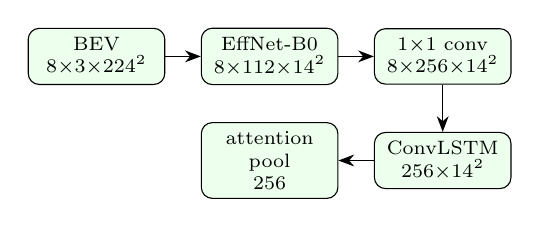
\begin{tikzpicture}[
  font=\scriptsize,
  n/.style={draw,rounded corners,minimum height=7mm,text width=15mm,align=center,fill=green!7},
  >={Stealth[length=2mm]},
  node distance=4.5mm
]
\node[n] (a) {BEV\\$8{\times}3{\times}224^2$};
\node[n,right=of a] (b) {EffNet-B0\\$8{\times}112{\times}14^2$};
\node[n,right=of b] (c) {$1{\times}1$ conv\\$8{\times}256{\times}14^2$};
\node[n,below=6mm of c] (d) {ConvLSTM\\$256{\times}14^2$};
\node[n,left=of d] (e) {attention pool\\$256$};
\draw[->] (a)--(b);
\draw[->] (b)--(c);
\draw[->] (c)--(d);
\draw[->] (d)--(e);
\end{tikzpicture}
\caption{Vision branch. Sekiz BEV karesi EfficientNet-B0 ile kodlanır, $1\times1$ convolution ile $256$ kanala indirgenir, ConvLSTM ile zamansal olarak bütünleştirilir ve uzamsal attention pooling ile tek bir $256$ boyutlu vektöre dönüştürülür.}
\label{fig:vision}
\end{figure}

Elde edilen özellik dizisi $\{F_t\}_{t=1}^{T}$ bir ConvLSTM'e beslenir. ConvLSTM, klasik LSTM gate'lerini convolution ile değiştirerek uzamsal yapıyı korur:
\begin{align}
i_t,f_t,o_t &= \sigma(W_{\{i,f,o\}} * [F_t, h_{t-1}]), \\
g_t &= \tanh(W_g * [F_t, h_{t-1}]), \\
c_t &= f_t \odot c_{t-1} + i_t \odot g_t, \quad h_t = o_t \odot \tanh(c_t).
\end{align}
Forget gate'in bias değeri $1$ olarak başlatılır; bu, eğitimin ilk adımlarında gradient akışını iyileştiren bilinen bir tekniktir. Zamansal bütünleştirme bu branch'in en kritik bileşenidir, çünkü bir engele yaklaşma hızı ya da birkaç kare boyunca süren bir yavaşlama eğilimi tek bir karede görünmez; yalnızca ardışık BEV karelerinin birlikte değerlendirilmesiyle ortaya çıkar. Son hidden state $h_T \in \mathbb{R}^{256\times14\times14}$, uzamsal bir softmax attention pooling ile tek bir $256$ boyutlu vektöre indirgenir. Attention pooling, sahnenin karara en çok katkı yapan bölgelerine ağırlık vererek sabit bir average pooling'den daha esnek bir özet üretir.

\subsection{State Branch: Ego-State Encoding}

State branch, her karede $21$ boyutlu bir sayısal öznitelik vektörü alır. Bu öznitelikler aracın anlık hızını ve hız bileşenlerini, dönüş açılarını, çevredeki araç ve yaya yoğunluğunu, hava koşullarını, karelerden türetilen ivme ve hız değişimini, durağanlık göstergesini ve öndeki engele ilişkin LiDAR ve bounding-box temelli betimleyicileri içerir. Tam liste Tablo~\ref{tab:ego}'de verilmiştir. Önemli bir nokta, bu skaler özniteliklerin tıpkısının temel modelde de kullanılmış olmasıdır; böylece temel model ile hibrit model arasındaki fark, skaler bilginin kendisinden değil, yalnızca BEV, image ve zamansal modellemenin eklenmesinden kaynaklanır ve karşılaştırma adil bir ablasyona dönüşür.

% TABLE - ego-features
\begin{table}[t]
\caption{State branch'inde kullanılan ego-state öznitelikleri}
\label{tab:ego}
\centering
\footnotesize
\begin{tabular}{@{}p{0.46\columnwidth}p{0.46\columnwidth}@{}}
\toprule
hız (km/sa) & hız bileşenleri $v_x, v_y, v_z$ \\
dönüş açıları (pitch, yaw) & 50 m içi araç sayısı \\
toplam NPC araç / yaya & hava: cloudiness, fog \\
durağanlık (ikili) & ivme $a_x, a_y, a_z$ \\
ivme büyüklüğü & hız değişimi $\Delta v$ \\
nesne risk skoru & öndeki nesne var / ortalı \\
ön LiDAR mesafesi & \\
\bottomrule
\end{tabular}
\end{table}

Bu $21$ boyutlu dizi bir GRU ile işlenir ve son hidden state $128$ boyutlu ego-state özetini oluşturur. GRU'nun recurrent yapısı, hız ve ivmenin pencere boyunca nasıl değiştiğini, örneğin bir yavaşlama ya da hızlanma eğilimini örtük olarak kodlar. Bu zamansal özet özellikle boylamsal kontrol için değerlidir, çünkü throttle ve brake kararları büyük ölçüde aracın o anki hız durumuna ve yakın geçmişteki ivme yönüne bağlıdır.

\subsection{Image Branch: Multi-Camera Encoding}

Image branch, karar karesine ait dört kamera görüntüsünü --- ön, sol-ön, sağ-ön ve arka --- $224\times224$ boyutunda ve ImageNet normalizasyonuyla alır. Dört görünümün tamamı, BEV branch'inden ayrı tutulan tek bir paylaşımlı EfficientNet-B1 örneğiyle kodlanır; yani backbone ağırlıkları görünümler arasında bağlıdır. Bu ağırlık paylaşımı, görece küçük veri kümesinde parametre verimliliği sağlar ve tüm kameraların aynı özellik uzayına eşlenmesini güvence altına alır. Her görünüm için backbone'un son convolution çıktısı global average pooling ile $1280$ boyutlu bir vektöre dönüştürülür, ardından doğrusal bir izdüşüm, ReLU ve dropout ile $256$ boyutuna indirgenir. Dört görünümün $256$ boyutlu özetleri art arda eklenerek $1024$ boyutlu image temsilini oluşturur. Akış Şekil~\ref{fig:image}'de özetlenmiştir.

Kamera akışı yalnızca karar karesinden alınır; image branch'i zamansal olarak modellenmez. Bu bilinçli bir tasarım kararıdır: kamera görünümlerini bir ConvLSTM ile zamansal olarak işleyen denemeler doğrulama kaybını düşürmüş, ancak test kümesine daha kötü aktarılmıştır (Bölüm~\ref{sec:results}). Etiketin pencerenin son karesinde tanımlı olması ve zamansal bağlamın zaten BEV ile ego-state branch'lerinden gelmesi, tek karar-karesini doğru indüktif önyargı kılar.

% FIGURE - image-branch
\begin{figure}[t]
\centering
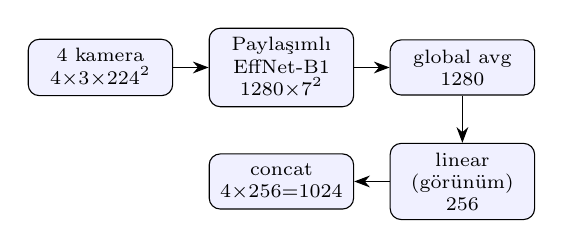
\begin{tikzpicture}[
  font=\scriptsize,
  n/.style={draw,rounded corners,minimum height=7mm,text width=16mm,align=center,fill=blue!6},
  >={Stealth[length=2mm]},
  node distance=4.5mm
]
\node[n] (a) {4 kamera\\$4{\times}3{\times}224^2$};
\node[n,right=of a] (b) {Paylaşımlı\\EffNet-B1\\$1280{\times}7^2$};
\node[n,right=of b] (c) {global avg\\$1280$};
\node[n,below=6mm of c] (d) {linear (görünüm)\\$256$};
\node[n,left=of d] (e) {concat\\$4{\times}256{=}1024$};
\draw[->] (a)--(b);
\draw[->] (b)--(c);
\draw[->] (c)--(d);
\draw[->] (d)--(e);
\end{tikzpicture}
\caption{Image branch. Dört kamera görünümü paylaşımlı bir EfficientNet-B1 ile kodlanır; her görünüm global average pooling ve doğrusal izdüşümle $256$ boyutlu bir özete indirilir ve dört özet birleştirilerek $1024$ boyutlu image temsili elde edilir.}
\label{fig:image}
\end{figure}

Image branch'inin BEV branch'inden ayrı bir backbone örneği kullanması da bilinçli bir karardır. Kamera görüntüleri doğal görüntü alanına aittir ve ImageNet ağırlıklarıyla iyi örtüşür; oysa BEV kanalları yükseklik, şiddet ve doluluktan oluşan, doğal görüntüden farklı bir alandır. İki modalitenin tek bir paylaşımlı backbone'a zorlanması, birinin lehine bir uzlaşmaya yol açardı; ayrı örnekler her modalitenin kendi özelliklerini serbestçe öğrenmesine olanak tanır. Image branch'inde backbone kapasitesi de deneysel olarak belirlenmiştir; EfficientNet-B0, B1 ve B3 karşılaştırmasında en iyi genel başarımı orta kapasiteli B1 vermiştir (Bölüm~\ref{sec:results}, Tablo~\ref{tab:ablation}).

\subsection{Late Fusion ve Çıkış Başlıkları}

Üç branch'in özetleri --- sırasıyla $256$ (BEV), $128$ (ego-state) ve $4{\times}256{=}1024$ (image) boyutlu vektörler --- art arda eklenerek $1408$ boyutlu bir füzyon temsili oluşturur. Bu temsil iki katmanlı bir fusion başlığından geçirilir: ilk doğrusal katman boyutu $256$'ya indirir, ReLU ve görece yüksek bir dropout ile düzenlileştirme uygular, son doğrusal katman ise üç ham skor üretir. Füzyonun bu noktada gerçekleşmesi, modelin kararı verirken üç modaliteyi birlikte değerlendirmesini, ancak her birinin temsilini bağımsız öğrenmesini sağlar. Üç ham skor, kontrol sinyallerinin doğal aralıklarına şu şekilde eşlenir:
\begin{equation}
\hat{b} = \sigma(s_b),\quad \hat{g} = \sigma(s_g),\quad \hat{d} = \tanh(s_d).
\end{equation}
Brake ve throttle için sigmoid bunları $[0,1]$ aralığına, steer için tanh ise $[-1,1]$ aralığına sıkıştırır. Bu seçim, çıkışları fiziksel sınırlar içinde tuttuğu için kontrol hedeflerinin ayrıca normalize edilmesini gereksiz kılar ve değerlendirmenin doğrudan fiziksel ölçekte yapılmasına imkân verir.

\subsection{Kayıp Fonksiyonu}

Eğitimde, kontrol sinyallerinin dengesiz yapısını telafi eden ağırlıklı bir ortalama kare hata kullanılır:
\begin{equation}
\mathcal{L} = \frac{1}{3B}\sum_{j=1}^{B}\sum_{k\in\{b,g,d\}} w_{j,k}\,(\hat{y}_{j,k}-y_{j,k})^2.
\end{equation}
Ağırlıklar şu kurala göre belirlenir: throttle için gerçek değer $0{,}01$'in üzerindeyse $w=2$, aksi hâlde $1$; steer için gerçek değerin mutlak büyüklüğü $0{,}1$'i aşıyorsa $w=4$, aksi hâlde $1$; brake için $w=1$. Bu ağırlıklandırma, çoğu karede sıfıra yakın olan steer ve throttle örneklerinin gradient'i bastırmasını engeller ve modeli aktif manevra anlarına, yani keskin dönüşlere ve belirgin gaz uygulamalarına odaklar.

\subsection{Kontrol Sinyalleri ile Modaliteler Arasındaki İlişki}
\label{sec:relation}

Üç kontrol sinyali iki bağımsız eksene ayrılır. Steer yanal kontroldür ve büyük ölçüde sahne geometrisine bağlıdır; şerit eğriliği ve yol yönelimi en doğrudan BEV doluluk haritasında ve kamera görünümlerinde görünür. Ego-state'teki yaw ve $v_y$ bileşenleri yalnızca dolaylı bir ipucu sunar. Dolayısıyla steer, uzamsal ve görsel modellemeden en çok yararlanması beklenen sinyaldir.

Brake ve throttle boylamsal ekseni oluşturur ve fiziksel olarak birbirini dışlar; araç aynı anda hem gaz hem fren uygulamadığı için iki sinyal negatif ilişkilidir. Brake kararı tipik olarak öndeki bir engelin ya da durma gereğinin varlığıyla tetiklenir ve bu durum BEV doluluk kanalında, ön LiDAR mesafesinde ve nesne risk skorunda kodludur. Throttle ise sürekli bir hızlanma kararıdır; aracın o anki hızına ve önün açık olup olmadığına bağlıdır, seyir ile hızlanma arasında birden çok çalışma noktasına yayıldığı için en güç kestirilen sinyaldir. ConvLSTM'in zamansal bütünleştirmesi özellikle bu boylamsal kararlar için belirleyicidir: bir engele yaklaşma hızı, frenlemenin ne zaman ve ne şiddette uygulanacağını tek bir kareden çok daha güvenilir biçimde belirler. Bu ilişkiler, Bölüm~\ref{sec:results}'deki ablasyon sonuçlarıyla deneysel olarak da doğrulanmaktadır.

% SECTION - DATASET AND EXPERIMENTAL SETUP
\section{Veri Seti ve Deneysel Kurulum}

\subsection{Veri Seti}

Deneyler, CARLA otopilotu ile toplanmış çok-modlu bir veri kümesi üzerinde yürütülmüştür \cite{immanuel_peter_2025}. Veri kümesi $30$ otopilot sürüşünden elde edilen senkron çok-modlu kareler içerir: çoklu RGB kameralar, anlamsal segmentasyon, $32$ kanallı LiDAR, iki boyutlu bounding-box etiketleri ve ego-state ile kontrol sinyalleri. Sürüşler farklı hava, gün ışığı ve trafik yoğunluğu koşullarını kapsar. Bu çalışmada dört kamera görünümü (ön, sol-ön, sağ-ön ve arka), LiDAR ve ego-state alanları kullanılmıştır.

Ham veriden iki türev temsil önceden hesaplanır. LiDAR taramaları yukarıda tanımlanan dönüşümle BEV dizilerine, kamera görüntüleri ise $224\times224$ boyutuna ölçeklenmiş dizilere çevrilir. Öznitelik mühendisliği aşamasında ön LiDAR mesafesi, bounding-box'lardan türetilen öndeki nesne göstergeleri, sezgisel bir nesne risk skoru ve sürüş bazında türetilen ivme ile hız değişimi öznitelikleri üretilir.

Veri, dosya düzeyinde bölünür. Resmî eğitim ve doğrulama dosyaları birleştirilip karıştırılır ve yüzde $85$/yüzde $15$ oranıyla eğitim ve doğrulamaya ayrılır; resmî test bölümü tümüyle ayrı tutulur. Dosya düzeyinde bölme, ardışık ve örtüşen pencerelerin bölünmeler arasına sızmasını engelleyerek başarımın iyimser tahmin edilmesini önler. $T=8$ pencere uzunluğu ve $2$ adımlık kayma ile pencereleme yapıldıktan ve eğitimde durağan pencerelerin yüzde $30$'u korunacak şekilde altörnekleme uygulandıktan sonra sırasıyla $16\,413$ eğitim, $2\,938$ doğrulama ve $3\,386$ test dizisi elde edilir. Ego-state ölçekleyici yalnızca eğitim verisi üzerinde uydurulur ve aynı istatistiklerle doğrulama ile teste uygulanır.

\subsection{Veri Artırma ve Normalizasyon}

Eğitimde üç artırma uygulanır. BEV'in yükseklik ve şiddet kanallarına küçük bir Gauss gürültüsü eklenir, aynı kanallara hafif bir parlaklık ölçeklemesi uygulanır ve yüzde $50$ olasılıkla yatay ayna çevirme yapılır. Ayna çevirme uygulandığında dünya tutarlılığını korumak için steer etiketi ile ego-state'teki $v_y$, yaw ve $a_y$ bileşenlerinin işaretleri ters çevrilir; kamera görüntüleri genişlik ekseninde aynalanır ve sol-ön ile sağ-ön görünümleri birbiriyle yer değiştirir. Yatay çevirme bu çalışmada özellikle önemlidir, çünkü sola ve sağa dönüşleri dengeleyerek steer dağılımındaki olası yön önyargısını giderir. Girdiler normalize edilir: ego-state için z-skor, BEV için veri kümesi istatistikleri, kameralar için ImageNet istatistikleri kullanılır. Kontrol hedefleri ise çıkış başlıklarının doğal aralıklarıyla örtüştüğü için olduğu gibi bırakılır.

\subsection{Eğitim Ayarları}

Model PyTorch \cite{Paszke19PyTorch} ile uygulanmış, temel model ise scikit-learn \cite{Pedregosa11Sklearn} ile eğitilmiştir. Eğitim hiperparametreleri Tablo~\ref{tab:hparam}'de, kullanılan donanım Tablo~\ref{tab:hw}'de özetlenmiştir. Optimizer olarak AdamW \cite{Loshchilov19AdamW} seçilmiş, batch normalization ve bias parametreleri için weight decay sıfırlanmıştır. Önceden eğitilmiş backbone'lar diğer modüllere göre on kat düşük öğrenme oranıyla güncellenir; böylece ImageNet'ten gelen genel görsel özellikler korunurken üst katmanlar göreve uyarlanır.

Early stopping, doğrulama kaybı sekiz dönem boyunca iyileşmediğinde eğitimi sonlandırır. Bu mekanizma, modelin aşırı uyum göstermeye başladığı noktayı yakalayarak en iyi doğrulama performansına karşılık gelen ağırlıkları korur. Uygulamada en düşük doğrulama kaybı on dokuzuncu dönemde elde edilmiş ve tüm değerlendirme bu kontrol noktasıyla yapılmıştır.

% TABLE - hyperparams
\begin{table}[t]
\caption{Eğitim hiperparametreleri}
\label{tab:hparam}
\centering
\footnotesize
\renewcommand{\arraystretch}{1.15}
\begin{tabular}{@{}ll@{}}
\toprule
\textbf{Parametre} & \textbf{Değer} \\
\midrule
pencere uzunluğu $T$ & 8 \\
pencere kayması & 2 \\
batch size & 16 (etkin 64) \\
gradient accumulation & 4 \\
optimizer & AdamW \\
öğrenme oranı (modüller) & $3\times10^{-4}$ \\
öğrenme oranı (backbone) & $3\times10^{-5}$ \\
weight decay & $1\times10^{-2}$ \\
learning rate schedule & cosine annealing \\
gradient clipping & 1,0 \\
mixed precision & bfloat16 \\
maksimum dönem & 30 \\
early stopping sabrı & 8 \\
en iyi dönem & 19 \\
\bottomrule
\end{tabular}
\end{table}

% TABLE - hardware
\begin{table}[t]
\caption{Deney donanımı}
\label{tab:hw}
\centering
\footnotesize
\renewcommand{\arraystretch}{1.15}
\begin{tabular}{@{}ll@{}}
\toprule
\textbf{Bileşen} & \textbf{Özellik} \\
\midrule
GPU & NVIDIA RTX 5090 \\
CPU & Intel Core Ultra 9 275HX \\
RAM & 64 GB \\
framework & PyTorch \\
\bottomrule
\end{tabular}
\end{table}

\subsection{Değerlendirme Metrikleri}

Her kontrol sinyali için üç metrik raporlanır. Belirleme katsayısı $R^2$, modelin açıkladığı varyans oranını verir ve $1$'e yaklaştıkça tahmin gücü artar. Ortalama mutlak hata MAE, tahminlerin gerçek değerlerden ortalama sapmasını fiziksel ölçekte ölçer. Kök ortalama kare hata RMSE ise büyük hataları daha ağır cezalandırarak uç sapmalara duyarlılık sunar. Genel skor, üç sinyalin $R^2$ değerlerinin eşit ağırlıklı ortalamasıdır.

Bu metriklerin yanında, başarımın bir sınıf dengesizliği yapaylığı olup olmadığını denetlemek için iki ek analiz yapılır. İlk olarak her sinyalin ne ölçüde aktif olduğu, yani sıfırdan belirgin biçimde farklı değer aldığı oran hesaplanır. İkinci olarak metrikler yalnızca aktif örnekler üzerinde yeniden hesaplanır. Aktif örneklerdeki $R^2$ değerinin genel $R^2$'ye yakın olması, yüksek başarımın çoğunlukla sıfır tahmin etmenin kolaylığından değil, gerçek sinyal genliğinin doğru kestiriminden kaynaklandığını gösterir.

% SECTION - RESULTS
\section{Bulgular}
\label{sec:results}

\subsection{Temel Model ile Karşılaştırma}

Temel model, Bölüm III'te tanımlanan skaler özniteliklerin tıpkısını kullanan, ancak BEV haritası, kamera görüntüleri ve zamansal modelleme içermeyen tek kareli bir MLP regresörüdür. Bu nedenle iki model arasındaki fark yalnızca uzamsal, görsel ve zamansal bileşenlerin katkısını yansıtır. Test başarımı Tablo~\ref{tab:main}'de karşılaştırılmıştır. Hibrit model genel $R^2$'yi $0{,}8605$'ten $0{,}9221$'e yükseltir. Kazanımın dağılımı dikkat çekicidir: en büyük iyileşme steer kanalında görülür ve $0{,}8044$'ten $0{,}9144$'e, yani yaklaşık on bir puanlık bir artışa karşılık gelir. Throttle $0{,}8248$'den $0{,}8758$'e, brake ise $0{,}9524$'ten $0{,}9759$'a yükselir. Bu desen, steer'in doğası gereği uzamsal ve görsel bilgiye en bağımlı sinyal olduğu yönündeki beklentiyi doğrudan destekler.

% TABLE - main-results
\begin{table}[t]
\caption{Test başarımı: temel model ve önerilen hibrit model}
\label{tab:main}
\centering
\footnotesize
\renewcommand{\arraystretch}{1.2}
\begin{tabular}{@{}llccc@{}}
\toprule
\textbf{Model} & \textbf{Hedef} & \textbf{$R^2$} & \textbf{MAE} & \textbf{RMSE} \\
\midrule
\multirow{4}{*}{Temel (skaler MLP)}
 & brake    & 0,9524 & 0,0295 & 0,1046 \\
 & throttle & 0,8248 & 0,0223 & 0,0794 \\
 & steer    & 0,8044 & 0,0470 & 0,0664 \\
 & \textbf{genel} & \textbf{0,8605} & 0,0329 & 0,0835 \\
\midrule
\multirow{4}{*}{\textbf{Hibrit}}
 & brake    & \textbf{0,9759} & 0,0172 & 0,0746 \\
 & throttle & \textbf{0,8758} & 0,0216 & 0,0654 \\
 & steer    & \textbf{0,9144} & 0,0266 & 0,0438 \\
 & \textbf{genel} & \textbf{0,9221} & \textbf{0,0218} & \textbf{0,0613} \\
\bottomrule
\end{tabular}
\end{table}

\subsection{Ablasyon: Bileşenlerin Katkısı}

Önerilen modelin her bileşeninin katkısını ayrıştırmak için Tablo~\ref{tab:ablation}'de iki bloklu bir ablasyon çalışması sunulmaktadır; tüm satırlar aynı $3\,386$ örneklik test kümesinde değerlendirilmiştir. Üst blok eklemeli kurulumu izler: yalnız skaler özniteliklerle çalışan temel modelden başlayarak sırasıyla BEV ile ego-state, ardından tek bir ön kamera ve son olarak dört kameralı image branch eklenir. Alt blok ise önerilen modelden her seferinde yalnızca tek bir bileşeni değiştirerek o bileşenin payını yalıtır.

Eklemeli blok, steer'in modaliteye en duyarlı sinyal olduğunu açıkça gösterir: BEV ile ego-state'in eklenmesi steer $R^2$'sini $0{,}8044$'ten $0{,}8599$'a, ön kameranın eklenmesi $0{,}9076$'ya taşır. Çok kameralı image branch ile birlikte en yüksek genel başarım olan $0{,}9221$ elde edilir. Ancak burada dikkatli bir okuma gereklidir: çok kameraya geçişin yararı backbone kapasitesinden bağımsız değildir. Alt blokta görüldüğü gibi, image backbone'u B1'den B0'a indirildiğinde çok kameralı modelin genel başarımı $0{,}9003$'e düşer; bu değer, tek ön kameralı B0 modelinin $0{,}9129$'unun dahi altındadır. Yani ek kameralar tek başına bir iyileşme getirmemekte, ancak yeterli backbone kapasitesiyle (B1) birleştiğinde değer kazanmaktadır. Bu, basit bir ``daha çok kamera daha iyidir'' çıkarımı yerine bir kapasite--görünüm etkileşimine işaret eder.

Backbone kapasitesi tek başına da belirleyicidir. B0, B1 ve B3 karşılaştırmasında genel başarım orta kapasiteli B1'de tepe yapar ($0{,}9003 < 0{,}9221 > 0{,}9053$); en büyük B3, görece küçük veri kümesinde aşırı uyum göstererek B1'in gerisinde kalır. Ayrıca B1, throttle $R^2$'sini diğer tüm yapılandırmaların takıldığı $\sim\!0{,}85$ bandından $0{,}8758$'e taşıyan tek bileşendir.

Alt bloğun son iki satırı, işe yaramayan iki yaygın sezgiyi belgeler. Image branch'ine zamansal bir ConvLSTM eklemek genel başarımı $0{,}9104$'e düşürür; bu kol doğrulama kaybını iyileştirse de test kümesine daha kötü aktarılır, yani zamansal görüntü modellemesi bir transfer cezası getirir. Önceden eğitilmiş backbone'lara daha agresif bir ince ayar uygulamak (öğrenme oranı çarpanını $0{,}1$'den $0{,}3$'e çıkarmak) steer'i $0{,}9179$ ile en yüksek değerine taşısa da throttle'ı $0{,}8529$'a düşürerek aşırı uyuma yol açar ve genel başarımı $0{,}9150$'de bırakır; bu da önerilen modelin $0{,}1\times$ backbone öğrenme oranının daha dengeli olduğunu gösterir.

% TABLE - ablation
\begin{table}[t]
\caption{Ablasyon: bileşenlerin test başarımına ($R^2$) katkısı. Üst blok eklemeli kurulum, alt blok önerilen modelden tek bileşen değişikliğidir. Önerilen yapılandırma kalın gösterilmiştir; tüm satırlar aynı test kümesindedir.}
\label{tab:ablation}
\centering
\footnotesize
\renewcommand{\arraystretch}{1.2}
\begin{tabular}{@{}lcccc@{}}
\toprule
\textbf{Konfigürasyon} & \textbf{brake} & \textbf{throttle} & \textbf{steer} & \textbf{genel} \\
\midrule
\multicolumn{5}{@{}l}{\textit{Eklemeli kurulum}} \\
Ego-state MLP (temel)            & 0,9524 & 0,8248 & 0,8044 & 0,8605 \\
BEV + ego-state                  & 0,9758 & 0,8385 & 0,8599 & 0,8914 \\
BEV + ego + ön kamera (B0)       & 0,9770 & 0,8542 & 0,9076 & 0,9129 \\
\textbf{BEV + ego + çok kamera (B1)} & \textbf{0,9759} & \textbf{0,8758} & \textbf{0,9144} & \textbf{0,9221} \\
\midrule
\multicolumn{5}{@{}l}{\textit{Önerilen modelden tek değişiklik}} \\
image backbone: B1 $\rightarrow$ B0       & 0,9751 & 0,8456 & 0,8802 & 0,9003 \\
image backbone: B1 $\rightarrow$ B3       & 0,9762 & 0,8555 & 0,8844 & 0,9053 \\
image dalına zamansal ConvLSTM            & 0,9765 & 0,8467 & 0,9082 & 0,9104 \\
agresif backbone ince ayarı (0,3$\times$) & 0,9742 & 0,8529 & 0,9179 & 0,9150 \\
\bottomrule
\end{tabular}

\vspace{3pt}
\parbox{\columnwidth}{\footnotesize Tüm değerler aynı $3\,386$ örneklik test kümesinde, tek tohum ve tek bölünmeyle elde edilmiştir; yapılandırmalar ön-kayıtlı bir faktöriyel tasarımla değil sıralı arama ile bulunmuştur.}
\end{table}

\subsection{Sınıf Dengesi ve Aktif-Örnek Analizi}

Üç sinyalin aktiflik oranları ile yalnızca aktif örneklerde hesaplanan $R^2$ değerleri Tablo~\ref{tab:active}'de verilmiştir. Brake örneklerinin yüzde $48{,}1$'i, throttle örneklerinin yüzde $48{,}8$'i aktiftir; dolayısıyla bu iki boylamsal sinyal dengeli bir dağılıma sahiptir ve yüksek $R^2$ değerleri bir dengesizlik yapaylığı değildir. Steer örneklerinin yalnızca yüzde $28{,}8$'i belirgin biçimde aktiftir, çünkü sürüşün büyük bölümü düz yolda geçer. Buna rağmen steer'in aktif-örnek $R^2$ değeri $0{,}9346$ ile genel steer $R^2$'sinin ($0{,}9144$) üzerindedir. Bu fark, $R^2$'nin varyansa göre normalize olmasından kaynaklanır: düz sürüşteki sıfıra yakın steer örnekleri çok düşük varyanslı olduğundan genel $R^2$'yi aşağı çeker; yalnızca belirgin manevra içeren aktif örneklere bakıldığında açıklanan varyans oranı yükselir. Yatay ayna çevirme artırımı bu yüksek steer başarımını besleyen bir etken olup ilgili mekanizma Bölüm~\ref{sec:discussion}'de tartışılmaktadır. Üç sinyalin aktif-örnek $R^2$ değerlerinin genel değerlere yakın kalması, raporlanan başarımın gerçek sinyal genliğinin doğru kestiriminden kaynaklandığını doğrular.

% TABLE - active-subset
\begin{table}[t]
\caption{Aktiflik oranları ve yalnızca aktif örneklerde $R^2$}
\label{tab:active}
\centering
\footnotesize
\renewcommand{\arraystretch}{1.2}
\begin{tabular}{@{}lccc@{}}
\toprule
\textbf{Hedef} & \textbf{Aktiflik} & \textbf{$n_{\text{aktif}}$} & \textbf{$R^2_{\text{aktif}}$} \\
\midrule
brake    & 48,1\% & 1628 & 0,9525 \\
throttle & 48,8\% & 1651 & 0,8517 \\
steer    & 28,8\% & 975  & 0,9346 \\
\bottomrule
\end{tabular}
\end{table}

\subsection{Niteliksel İnceleme}

Tahmin ile gerçek değerlerin saçılımı Şekil~\ref{fig:scatter}'de gösterilmiştir. Steer kanalı dar bir köşegen bandı boyunca toplanır ve üç sinyal arasında en düşük RMSE değerine sahiptir; bu, modelin yanal kontrolü tutarlı biçimde kestirdiğini gösterir. Brake kanalı iki kutuplu bir yapı sergiler: noktaların büyük çoğunluğu sıfır civarında ve tam fren bölgesinde toplanır, modelin bu iki kümeyi büyük ölçüde doğru ayırdığı görülür. Sıfır ile tam fren arasındaki kısmi frenleme bölgesinde ise saçılma artar, yani modelin en belirsiz olduğu yer yumuşak frenleme rejimidir. Throttle kanalında gerçek değerlerin yaklaşık $0{,}85$ civarında bir doygunluk bandı oluşturduğu dikkat çeker. En büyük tahmin hataları bu doygunluk bölgesinde yoğunlaşır; model yüksek gaz değerlerinin bir kısmını olduğundan düşük kestirir. Bu gözlem, throttle'ın neden en zayıf tahmin edilen sinyal olduğunu somut biçimde açıklar.

% FIGURE - predictions
\begin{figure}[t]
\centering
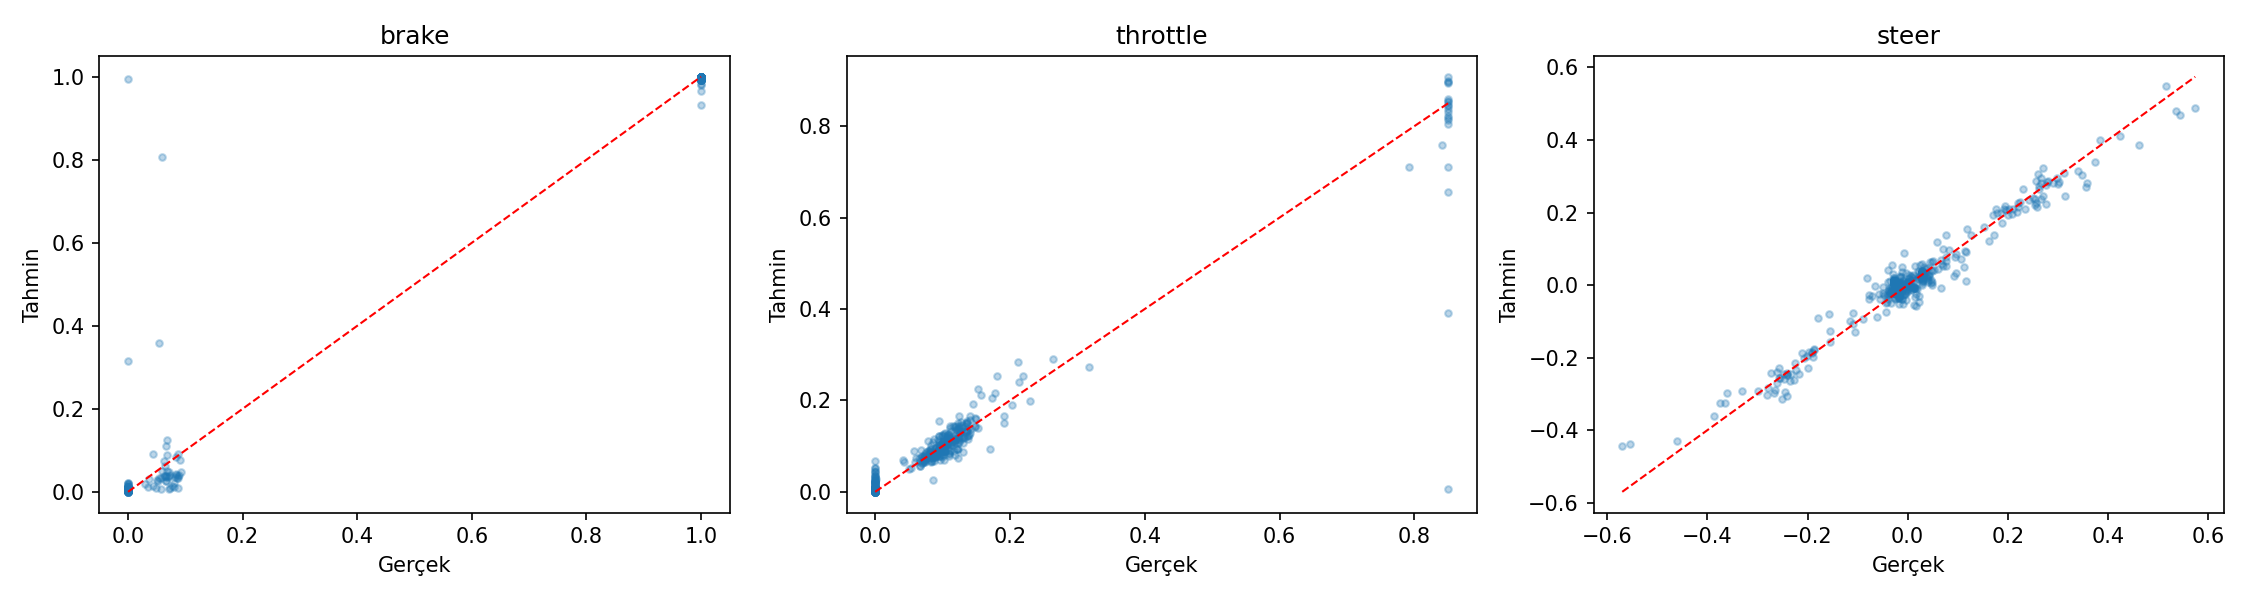
\includegraphics[width=\columnwidth]{predictions.png}
\caption{Test kümesinde tahmin ile gerçek değerlerin saçılımı. Soldan sağa brake, throttle ve steer. Kırmızı kesik çizgi ideal $y=x$ doğrusunu gösterir.}
\label{fig:scatter}
\end{figure}

% SECTION - DISCUSSION
\section{Tartışma}
\label{sec:discussion}

Bulgular, Bölüm~\ref{sec:relation}'de öne sürülen modalite ile kontrol ilişkilerini açık biçimde doğrulamaktadır. Steer kanalındaki büyük iyileşme, yanal kontrolün bir geometri-algılama görevi olduğu ve BEV ile kamera bilgisinden en çok bu sinyalin yararlandığı düşüncesini destekler. Temel modelin elindeki yaw ve $v_y$ gibi skaler vekiller yolun şeklini doğrudan göremedikleri için sınırlı kalmıştır; oysa hibrit model, BEV doluluk haritası ve kamera görünümleri sayesinde şerit eğriliğini doğrudan algılayabilmektedir.

Steer'in az sayıda aktif örneğe rağmen yüksek başarıma ulaşması iki etkenle açıklanır. Birincisi veri artırmadır: yatay ayna çevirme, her sürüş karesinin sola ve sağa dönüş karşılığını birlikte üreterek etkin manevra çeşitliliğini artırır ve veri kümesindeki olası yön önyargısını ortadan kaldırır; böylece model görece seyrek olan dönüş anlarını dengeli biçimde öğrenir. İkincisi bir ölçüm etkisidir: aktif steer örneklerindeki $R^2$ ($0{,}9346$) genel steer $R^2$'sinin ($0{,}9144$) üzerindedir, çünkü $R^2$ varyansa göre normalize olur ve düz sürüşteki sıfıra yakın, düşük varyanslı örnekler genel değeri aşağı çeker. Temel modelin böyle bir uzamsal artırımdan yararlanamaması, iki model arasındaki steer farkını daha da büyütmektedir.

Throttle'ın en zayıf sinyal olması beklenen bir sonuçtur. Throttle aktif olduğu sürece süren ve seyir ile hızlanma arasında çok-modlu bir dağılım sergileyen sürekli bir karardır; üstelik veride yaklaşık $0{,}85$ değerinde doyuma ulaşır. Bu doygunluk bölgesi, modelin tek bir gözlemden hangi yüksek gaz değerinin uygulanacağını belirlemesini güçleştirir. Yine de image backbone'unun B1'e yükseltilmesi, throttle $R^2$'sini diğer tüm yapılandırmaların takıldığı $\sim\!0{,}85$ bandından $0{,}8758$'e taşıyan tek müdahale olmuştur; bu, daha güçlü görsel özelliklerin gözlemlenebilirlik tavanını bir miktar yukarı ittiğini, ancak $0{,}90$ eşiğini kıramadığını gösterir. Brake ise hem yüksek $R^2$ hem de yüksek aktif-örnek başarımıyla en güvenilir tahmin edilen sinyaldir; modelin en belirgin zorlandığı yer, sıfır ile tam fren arasındaki yumuşak frenleme rejimidir. Güvenlik açısından bu rejimin daha iyi modellenmesi öncelikli bir iyileştirme alanı olarak öne çıkar.

Ablasyon, mimari kararlara ilişkin üç ek çıkarım sunar. Birincisi, image backbone kapasitesi orta boyutta (B1) en iyi sonucu verir; daha büyük B3 görece küçük veri kümesinde aşırı uyum göstererek geriler, dolayısıyla ``daha büyük her zaman daha iyi'' varsayımı bu ölçekte geçerli değildir. İkincisi, çok kameralı girdinin yararı backbone kapasitesinden ayrılamaz: ek kameralar yalnızca yeterli kapasiteyle (B1) birlikte değer kazanır, zayıf bir backbone'la (B0) tek ön kameranın dahi gerisine düşer. Üçüncüsü, kamera koluna zamansal modelleme eklemek doğrulama kaybını düşürse de test başarımını geriletir; bu transfer cezası, zamansal bağlamın zaten BEV ve ego-state branch'lerince taşınması ve etiketin tek bir karede tanımlı olmasıyla tutarlıdır.

Çalışmanın açıkça belirtilmesi gereken sınırları vardır ve bu sınırlar bir sonraki tez çalışmasının yönünü doğrudan belirler. En önemlisi, değerlendirme open-loop koşullarda yapılmıştır; yani model, kaydedilmiş bir test kümesi üzerinde tek adımlık tahminlerle ölçülmüştür. Literatürün gösterdiği gibi open-loop hata, gerçek sürüş kalitesiyle yalnızca zayıf ilişkilidir \cite{CodevillaOffline18}; dolayısıyla yüksek $R^2$ doğrudan iyi sürüş anlamına gelmez. İkinci olarak, ego-state vektörü çevredeki araç sayısı, hava parametreleri ve bounding-box'lardan türetilen göstergeler gibi, gerçek bir araçta ancak ek bir algılama katmanıyla elde edilebilecek ayrıcalıklı bilgiler içerir; bu nedenle başarım ayrıcalıklı girdi varsayımı altında değerlendirilmelidir. Üçüncü olarak, sonuçlar tek bir tohum ve tek bir bölünme ile elde edilmiştir, dolayısıyla çoklu tohumla yürütülecek bir varyans analizi sonuçların kararlılığını güçlendirecektir.

% SECTION - CONCLUSION
\section{Sonuç ve Gelecek Çalışmalar}

End-to-end otonom sürüşte kontrol üretmenin iki temel yolu vardır: sinyalleri doğrudan kestirmek ya da bir trajectory tahmin edip onu bir denetleyiciyle kontrole çevirmek. Bu çalışma birinci yolu izlemiş ve tüm sensörleri kullanan bir füzyon mimarisi kurulduğunda brake, throttle ve steer'in doğrudan ne ölçüde kestirilebileceğini araştırmıştır. CARLA otopilot verisi üzerinde, BEV vision branch, ego-state branch ve çok kameralı image branch'inden oluşan modüler bir hibrit model önerilmiş; bu model yalnızca skaler özniteliklerle eğitilen güçlü bir MLP temel modelini genel $R^2$'de $0{,}8605$'ten $0{,}9221$'e taşımıştır. Kazanımın büyük bölümü, uzamsal ve görsel modellemenin en belirleyici olduğu steer kanalında yoğunlaşmıştır. Tek değişkenli bir ablasyon çalışması, bu kazanımın çok kameralı image branch ile orta kapasiteli (B1) bir görüntü backbone'unun etkileşiminden geldiğini; zamansal görüntü modellemesi ve daha agresif ince ayar gibi sezgisel eklemelerin ise transfer cezası ve aşırı uyum nedeniyle yarar getirmediğini göstermiştir. Aktif-örnek analiziyle, raporlanan başarımın bir dengesizlik yapaylığı olmadığı üç sinyal için ayrı ayrı gösterilmiştir.

Bu çalışmanın asıl değeri, ulaşılan yüksek open-loop başarımın ötesinde, doğrudan üç-kontrol kestirimi yaklaşımının sınırlarını somut biçimde ortaya koymasıdır. Üç sinyalin tek bir ağda aynı anda öğrenilmesi, istatistiksel yapıları birbirinden farklı olduğu için zordur ve yüksek $R^2$ değerleri bile doğrudan kontrol paradigmasının bilinen kırılganlıklarını ortadan kaldırmaz. Modelin kendi hatalarının zincirleme büyümesine açık olması, ayrıcalıklı girdilere dayanması ve trajectory düzeyinde bir düzeltme katmanından yoksun olması, closed-loop ve gerçek dünya koşullarında başarımın düşmesine yol açabilecek etkenlerdir. Literatürdeki eğilim de bu gözlemi destekler: çok-modlu füzyon çalışmaları doğrudan kontrol yerine waypoint kestirimine ya da daha sınırlı kontrol alt kümelerine yönelmiş, robustluğu öncelemiştir. Bu çalışmada görülen eksiklikler, planlanan tez çalışmasının doğrudan odağını oluşturacaktır.

Gelecek çalışmalar üç yönde ilerleyecektir. İlk olarak model CARLA döngüsünde sürdürülerek route completion ve ihlal temelli closed-loop metriklerle değerlendirilecek; böylece open-loop başarımın gerçek sürüşe ne ölçüde aktarıldığı ölçülecektir. İkinci olarak ayrıcalıklı ego-state özniteliklerinin çıkarıldığı, yalnızca araç içi sensörlere dayanan bir sürüm eğitilerek bu bilginin katkısı ayrıştırılacaktır. Üçüncü olarak doğrudan kontrol ile waypoint kestirimini birleştiren melez bir çıkış tasarımı ve çoklu tohumla güven aralıkları araştırılacaktır.

% SECTION - REFERENCES
\bibliographystyle{IEEEtran}
\bibliography{refs}

\end{document}
